\documentclass[]{article}
\usepackage[T1]{fontenc}
\usepackage[utf8]{inputenc}
\usepackage{color}
\usepackage{titlesec}
\usepackage{hyperref}
\usepackage{float}
\usepackage{datetime}
\usepackage{graphicx}
\usepackage{amsmath}
\usepackage{amsfonts}
\usepackage{attachfile}
\usepackage[margin=3cm]{geometry}
\graphicspath{{./resources}}
\hypersetup{
	colorlinks=true,
	linktoc=all,
	linkcolor=blue,
}

\title{Analysis of natural language complexity used by open-source developers\\ \large Introduction to Natural Language Processing}
\author{Komlichenko Ilya, Krzemiński Piotr, Monicz Kamil, \\Piotrowska Weronika, Wojnarowski Marcin}
\date{\monthname, \the\year}
	
\newcommand{\code}[1]{\texttt{#1}}
\newcommand{\figref}[1]{{(Fig. \hypersetup{linkcolor=blue}\ref{#1})}}

\begin{document}

\maketitle

{\hypersetup{linkcolor=black}\tableofcontents}
\newpage


\section{Motivation}

In order to improve our NLP skills, we are going to complete simple natural language analysis. The topic of choice should be close to our hearts so we stay engaged throughout the project. In addition, the source data should be freely accessible, so it is easy to work with. And so, our analysis will focus on the natural language complexity used by developers of various programming languages who contribute to open-source platforms (such as GitHub).

We hypothesize that language with a lower barrier of entry (such as Python) will exhibit a lower natural language complexity than languages that expect a higher level of expertise (such as C). Additionally, we are aware of different demographics of programming languages thus expect scientific/research focused languages (such as Julia) programmers will naturally use a more complex natural language to express ideas/problems.

In the end the following set of programming languages was chosen:

\begin{enumerate}
    \item Python
    \item C
    \item JavaScript
    \item Golang
\end{enumerate}

We believe this subset will represent a wide range of kinds of programmers: Python used by beginners/scientific community, C used by low level developers, JavaScript used by everyone, and Golang used by modern system's programmers. Thus they have a different target demographic so we believe it should show some noticeable differences. Another reason this subset was chosen is the availability of resources: these language are quite popular therefore much data is present for it in GitHub (discussed in greater detail in section \ref{scraping_procedure}).

\section{Functionalities}

After scrapping the data, we are planning to perform following operations in order to give us a more complete insight

\begin{enumerate}
    \item Basic text analysis -- this includes average length of sentences, average length of words, most common word occurring etc. We are expecting developers of more complex programming languages to use more sophisticated language in the reported issues, this includes less grammar mistakes, longer sentences and words.

    \item Frequency of passive sentences -- in order to identify passive sentences we will use Part Of Speech tagging (POS). In English, a passive sentence can be defined by the place of the verb in the sentence and the form of this verb. We suspect the data to have high frequency of passive sentences, as it describes development issues.

    \item Flesh-Kincaid Grade Level -- Flesch-Kincaid grade is an objective numerical description of how hard a passage is to read in the English language. The final score indicates the US education grade level, thus higher score means a more advanced usage of the language. By evaluating the grade level, we can determine the whether the text is readable to an average, non-developer person.

          \[0.39\left(\frac{\text{total words}}{\text{total sentences}}\right) + 11.8\left(\frac{\text{total syllables}}{\text{total words}}\right) - 15.59\]

    \item Flesh readability score -- similarly to Flesh-Kincaid Grade Level, the Flesch reading score quantifies the ease of reading of a passage. Higher score indicates that the material is easier to read. We compute the score as follows:

          \[206.835 - 1.015\left(\frac{\text{total words}}{\text{total sentences}}\right) - 84.6\left(\frac{\text{total syllables}}{\text{total words}}\right)\]
\end{enumerate}

We hope that after obtaining this data, there will be interesting conclusions that there exists dependency between a developer's primary programming language and the natural language he or she uses when describing issues on GitHub.

\section{Data sourcing}

The linguistic data will be primarily scraped from the GitHub issues, where developers, using natural language, often describe bugs or feature requests related to some piece of software. And since the code there is publicly available, it is easy to assign a specific programming language to it.

\subsection{Text processing}

Every issue will be assigned a complexity/readability score based on industry-standard algorithms and bucketed into their respective programming language. For example, one could compute Flesch-Kincaid Grade Level or check the frequency of passive sentences.

\subsection{Scraping procedure} \label{scraping_procedure}

Using the official GitHub API we first fetch a list of users which we want to examine. To improve the quality of issues which we will be later studying, we made an assumption that GitHub users with more followers in general write issues of higher quality. We intuitively correlate higher followers count with a greater professionalism and higher activity on the platform. For each programming language a list of top 1000 (in terms of amount of followers) users with at least 170 followers\footnote{170 followers was chosen as the cutoff because it was the argmax such that all four programming languages have at least 1000 users each} was downloaded. An additional reason as to why the previously mentioned subset of languages was chosen is that these (unlike other languages which we had wished to investigate, such as purely scientific programming languages) do have a 1000 users with a reasonable amount of followers. Only personal accounts where taken into account, so organizations were filtered out since they represent more than a single person. A user was considered to be a $\mathbf P$ language programmer if majority of their repositories are written in $\mathbf P$\footnote{\href{https://docs.github.com/en/search-github/searching-on-github/searching-users\#search-by-repository-language}{Quoting the GitHub documentation}: "{\it \code{language:javascript} users [...] with a majority of their repositories written in JavaScript.}"}. Thus it is important to remember that a single developer could be possibly writing in other languages as well, or even could be overlapping with other classes we are investigating. It is rare that a developer knows and uses only a single programming language.

Afterwards, once we have a list of users (in total 4000 users) we proceed to fetching issues written by them. Top 100 issues created by a given user were downloaded. Only the body of the posted issue is saved, the thread that follows is ignored. Issues are ranked by the amount of interactions\footnote{An interaction consists of either a comment or a reaction} that they have received, thus top 100 issues refer to top 100 most active issues. Here, we make a similar assumption that more active issues correlate with a higher quality of natural language, for instance an RFC with naturally generates more traffic.

Finally, the gathered data is saved to a \code{csv} file containing the original author, their programming language, and the body of the issue. Since not every user had 100 issues, the final amount of scaped was 233,686 (where the upper bound is 400,000 if every user had 100 issues). We believe this is a very comfortable amount and even if after cleaning we will lose 50\%, this still will be enough.

\subsubsection{Technical details}

Scraper was written in the \href{https://www.rust-lang.org/}{Rust} programming language using the \href{https://github.com/XAMPPRocky/octocrab}{octocrab} library which wraps the official GitHub API. For all requests GitHub's search API was used, which has an unfortunate limit of 30 requests per minute. In each search call 100 items can be retrieved thus the whole scraping procedure spends $\frac{400000}{100 \cdot 30} = 133.(3)$ minutes on waiting for the limit rate alone. The scraper can be found in section \ref{attachments}.

\subsection{Cleaning up the data}

The previously scraped raw data contains a lot of noise, thus it has to be cleaned up. GitHub issues use markdown a text format which is a super-set of HTML, it allows for simple text formatting. Them being in a standardized format means we are able to parse them and work on their AST. For each body of an issue the following steps are taken:

\begin{enumerate}
    \item Parse into markdown AST
    \item Recursively walk the tree and skip tokens that are of non-interest (block code, inline code, links, images, etc.)
    \item Serialize the AST back to a visual rendered string form without the skipped tokens
\end{enumerate}

After these steps we are left with a much cleaner string representation of an GitHub issue. However, some additional steps have to be taken with the markdown cleaning due to limitation of the parsing markdown library and due to GitHub-specific features. Namely the following things were removed: hashtags (on GitHub they reference a different issue/pull request), unclosed code blocks, HTML comments (often appear in GitHub as issue templates), and inline URLs. Lastly we remove repetitive whitespace.

Now that we have clean utf-8 encoded text, we proceed to classify the content to its natural language. Since we are only interested in issues written in English we have to discard all issues written in a different natural language (for example chinese which was a common appearance). To do that a pre-trained model for Meta's \href{https://fasttext.cc/}{\code{fasttext}} NLP library. Given a string it classifies the natural language in which the text was written in. From there we filter in only those that were classified as english. Finally, if the cleanup content is not empty we save this entry into a new \code{csv} file.

Unfortunately, as we expected the final corpus is not perfect. Because of the human factor, we cannot guarantee that we removed all of the noise. For instance, someone could've written some code without wrapping it into code blocks or an inline code span. Thus we expect to still see some unwanted text in to final corpus. The dataset is unfortunately too large for us to manually clean it up. However we hope to be affected by these issues much less after choosing top users which should provide a higher quality of issues with regards to formatting. As seen on Fig. \ref{fig:cleaning-example} (in order of appearance) code blocks are removed, inline code is removed, non-english is discarded, and markdown formatting is removed to extract just the visual text.

\subsubsection{Technical details}

The data cleaner was written in Python using the previously mentioned library \code{fasttext}, standard dataframe tool \code{pandas}, and a markdown parser \code{mistletoe}. This process is much faster as it operates on local data. The data cleaner can be found in section \ref{attachments}.

\begin{figure}[H]
    \centering
    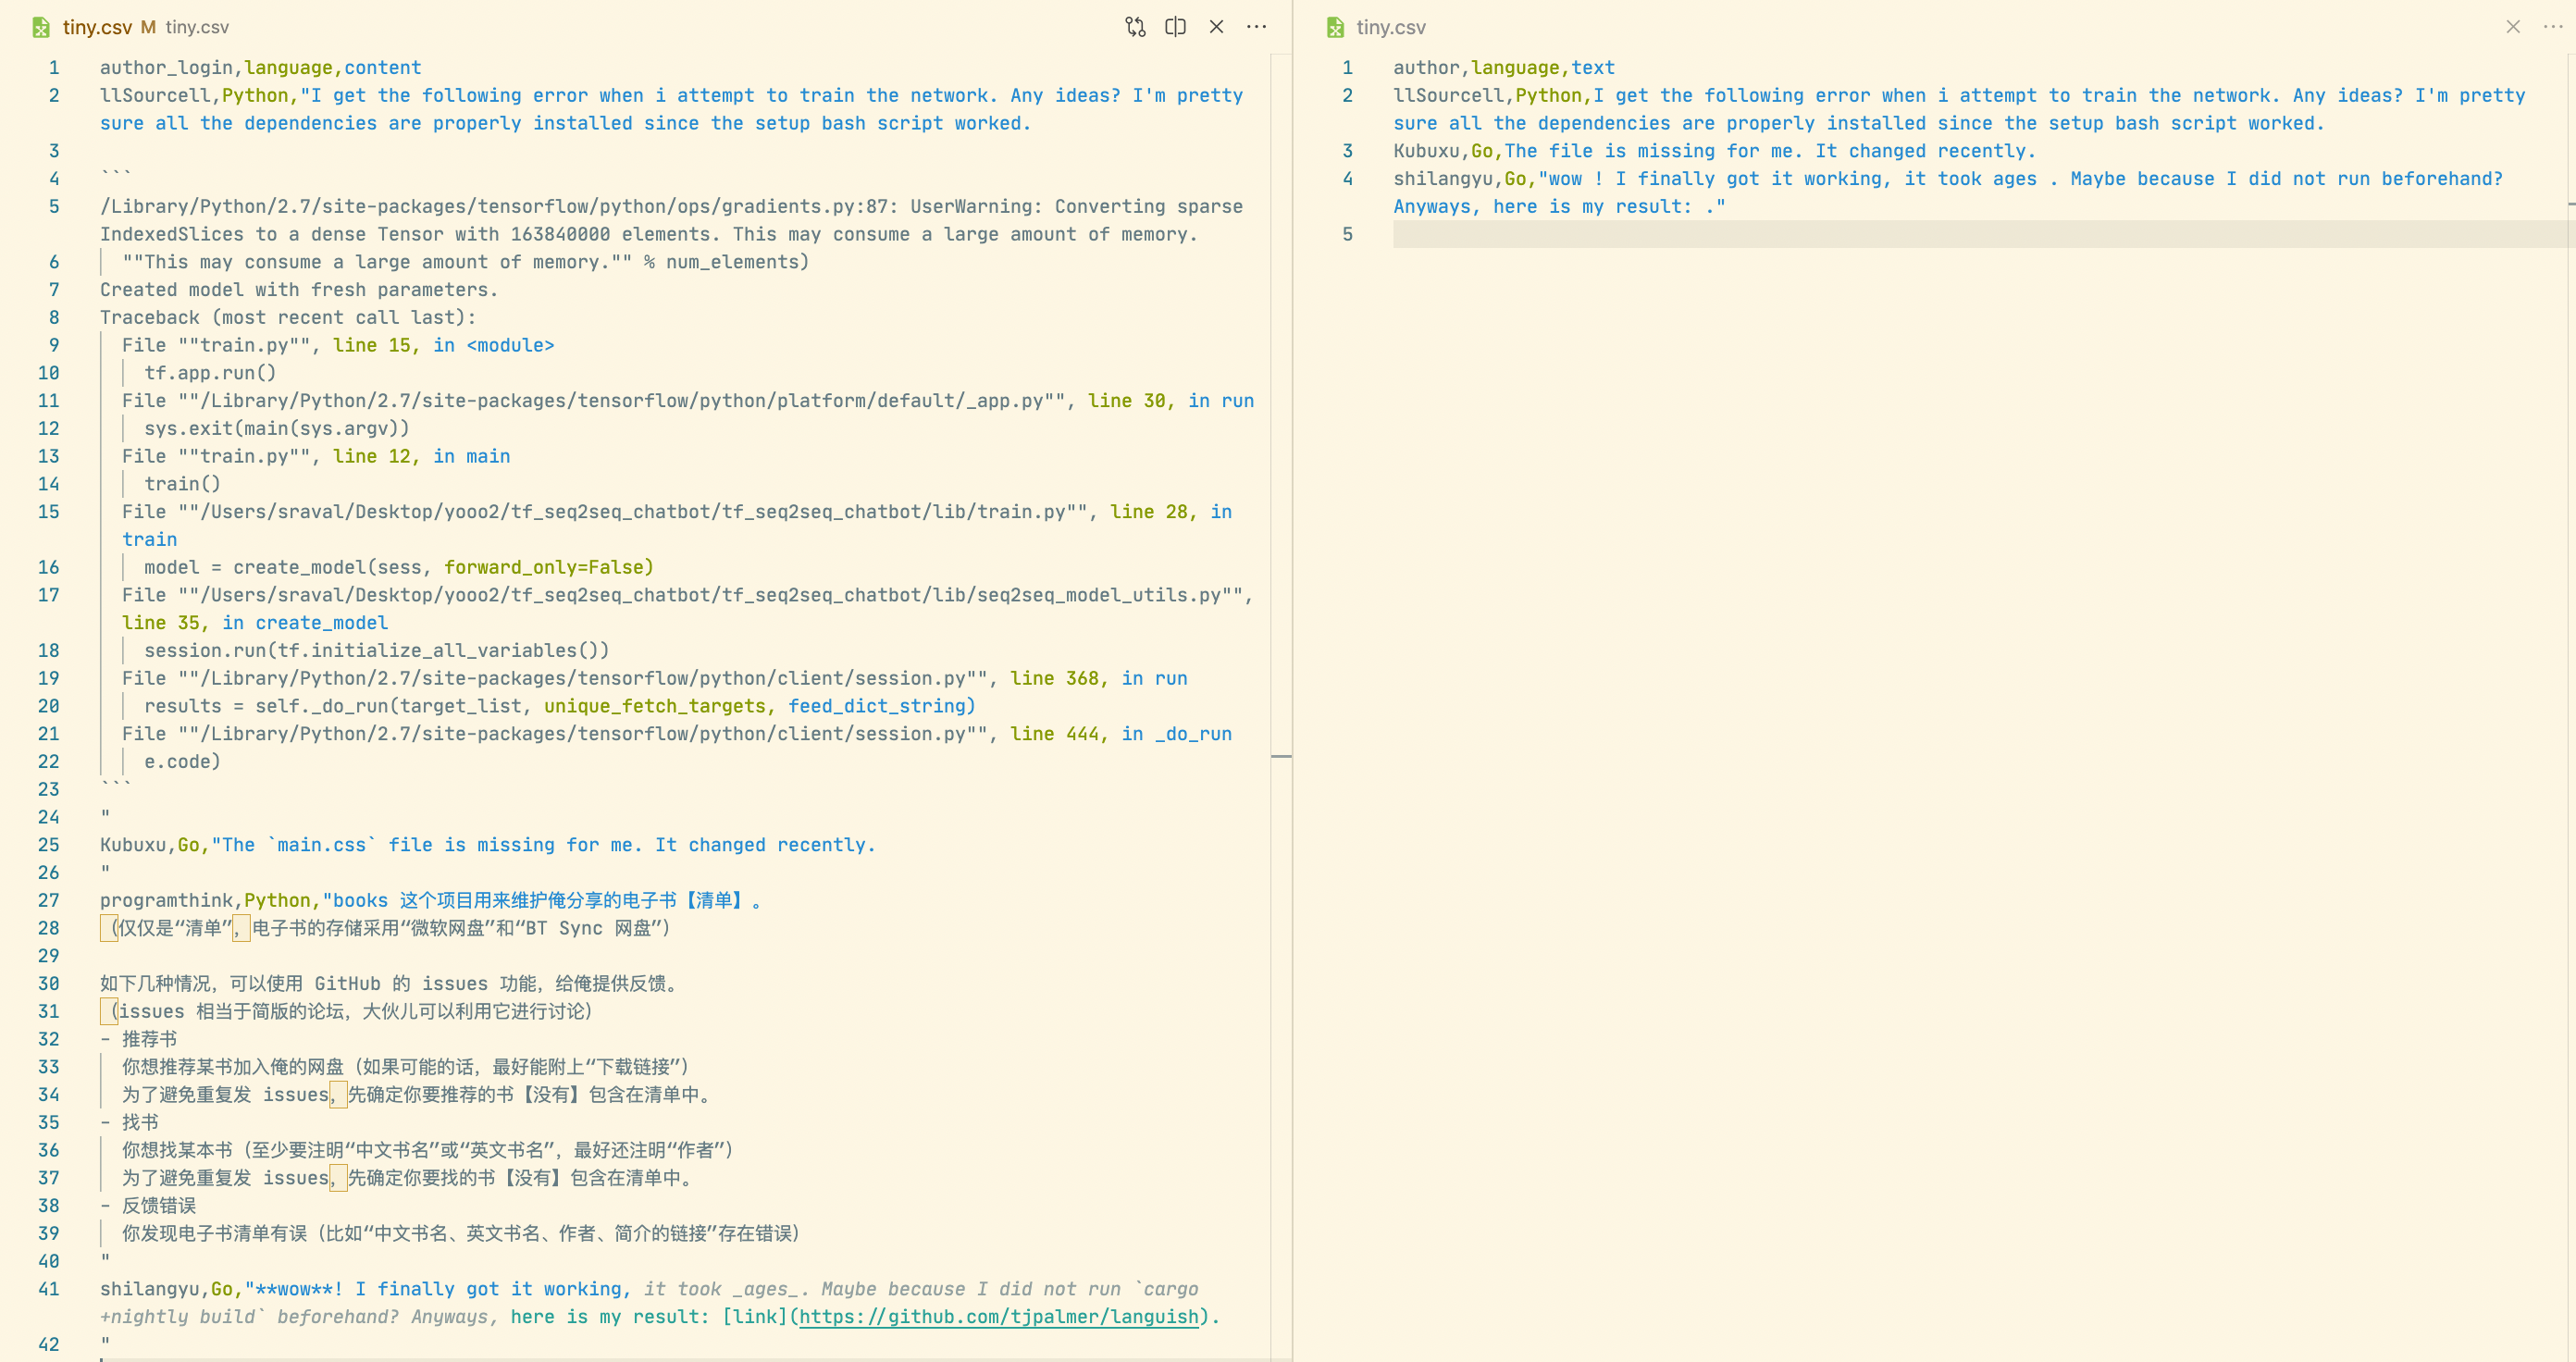
\includegraphics[width=1\textwidth]{cleaning-example.png}
    \caption{A sample example before (left) and after (right) cleaning of a csv file of the scraped issues.}
    \label{fig:cleaning-example}
\end{figure}

\subsection{Final corpus}

After cleaning we were left with 190643 instances, which means 18.4\% of instances were discarded. This is a very comfortable amount of data to make some analysis and draw some meaningful conclusions. On the other hand, the final corpus is as much as 67.2\% smaller (77MB vs. 235MB text csv) than the raw one, which shows that there was a lot of noise present and was successfully removed. But as mentioned before, there are still some false negatives left which we were able to identify when skimming the final corpus, thus it must be kept in mind during further analysis.

\section{Results}

Throughout the analysis we operated on three types of data:

\begin{enumerate}
    \item {\bf Text} -- String, "Raw" cleaned up text from the previous scraping+cleaning steps
    \item {\bf Tokenized text} -- List of strings, {\bf Text} but tokenized to individual tokens
    \item {\bf Normalized text} -- List of strings, {\bf Tokenized text} but normalized. That is, made lowercase, removed punctuation, removed stopwords.
\end{enumerate}

\subsection{Basic text analysis}

\begin{enumerate}
    \item Average text length

          This graph presents average length (in terms of words) of an issue description. We can observe that this value is similar for every analyzed class. Here C has the smallest average of 76 words, and Go has the largest with 81.5 words.


          \begin{figure}[H]
              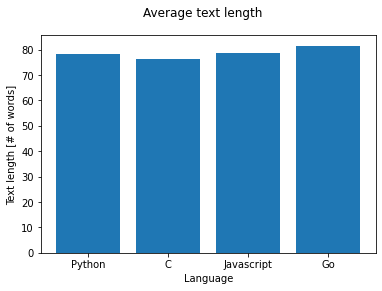
\includegraphics[width=8cm]{avg_len.png}
              \centering
          \end{figure}

    \item Average lexical diversity of a single issue

          This value is the average lexical diversity of a single issue. This value is obtained by dividing the cardinality of the set of all normalized words by the total number of words in a single issue. The value is then averaged for each class. We can observe no meaningful differences.

          \begin{figure}[H]
              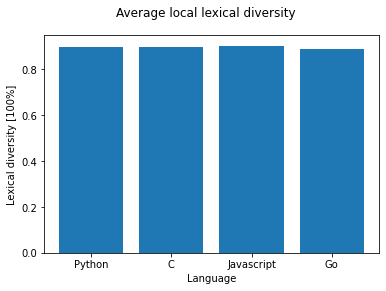
\includegraphics[width=8cm]{lex_div_single.png}
              \centering
          \end{figure}

    \item Total lexical diversity

          This value is the lexical diversity of all issues among the language. It is obtained by dividing the cardinality of the set of normalized words by the total number among all words in all issues per class. Here the situation is different, C shows an almost 1.5\% greater lexical diversity than Javascript and Golang. This could be due to the fact that C discussions often involve mentions of more cryptic library names, compiler flags, syscalls, etc. On the other hand, in the Golang and Javascript ecosystem things are often named using the natural language and thus blending in more uniformly into English which then do not increase the lexical diversity.

          \begin{figure}[H]
              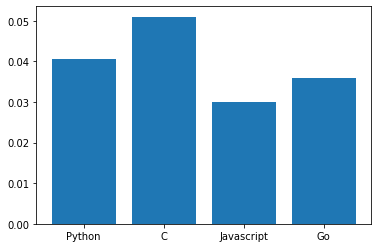
\includegraphics[width=8cm]{lex_div_total.png}
              \centering
          \end{figure}

    \item Average word length

          This is the average word length for every language. We can observe that this value is similar among all classes. C and Golang show a higher average, but the difference is too small to have any statistical significance. The average of slightly above 4 aligns with the english average of 4.7 \cite{letterfreq}.

          \begin{figure}[H]
              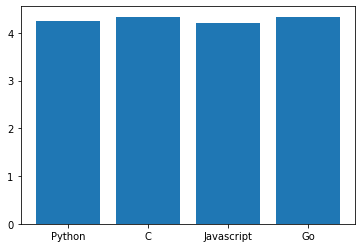
\includegraphics[width=8cm]{word_len.png}
              \centering
          \end{figure}

    \item Fraction of words over some longer length

          Here is the fraction of words over $\{8, 9, 10, 11\}$ characters long used in all issue descriptions among all languages. For the tested lengths, Javascript shows a lower percentage of longer words than other classes. C and Go equally exert a higher frequency of longer words compared to other classes.

          \begin{figure}[H]
              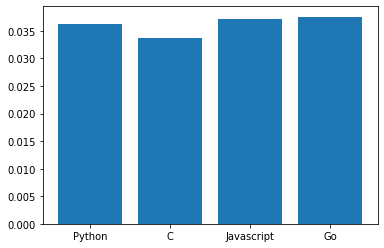
\includegraphics[width=8cm]{long_words.png}
              \centering
          \end{figure}

\end{enumerate}

\subsection{Frequency distributions}

In this section, we present the frequency distribution of tokens in the text. We can see the most common words used, as well as the cumulative value of this words.

\begin{enumerate}

    \item Python

          In Python, the most common words are would, like, code, use and using. Given over 2 900 000 tokens in the text, top 20 words make up to 37\% of the whole data.

          \begin{figure}[H]
              \includegraphics[width=8cm]{freq_Python.png}
              \centering
          \end{figure}

    \item C

          In C language, the most common words used are would, file, like, use and code. We can see that, given over 2 600 000 tokens in the text, top 20 words made up to 34\% of the total text.

          \begin{figure}[H]
              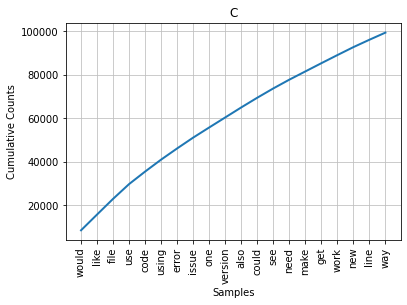
\includegraphics[width=8cm]{freq_C.png}
              \centering
          \end{figure}

    \item JavaScript

          In JavaScript, the most common words are would, like, use, using, could. Given 3 700 000 tokens in the whole text, top 20 words make up to over 40\% of the whole data.

          \begin{figure}[H]
              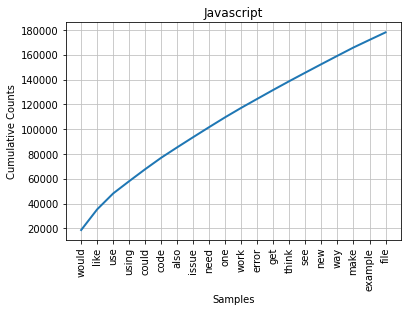
\includegraphics[width=8cm]{freq_Javascript.png}
              \centering
          \end{figure}

    \item Golang

          In Go, most common words are would, like, go, use, using. Given over 4 500 000 tokens, the top 20 make up to 40\% of the whole text.

          \begin{figure}[H]
              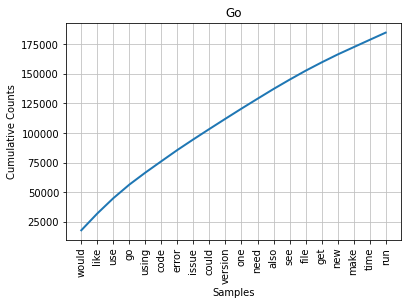
\includegraphics[width=8cm]{freq_Go.png}
              \centering
          \end{figure}


\end{enumerate}

We can observe that among all languages, issue comments contain variations of words \emph{would} and \emph{use}. We considered adding more stop words, but new common words kept surfacing which put us back to where we started. The most informative feature is that the word "\emph{file}" appears much less often in issues posted by Javascript developers in contrast to it being mentioned very often by C developers. This reflects the nature of the programming languages where C code manipulates files very often while Javascript being constrained to the browser does not have direct access to files.

Another interesting word which was investigated closely is the common appearance of \emph{go} in issues posted by golang developers. Displaying the concordance of the word \emph{go} within issues from the Golang class revealed something interesting,

\begin{verbatim}
Displaying 25 of 11503 matches:
nning tests works running tests godep go test failes find easy way send health
ders happy work think right direction go currently supported dns provider goog
s menu opened file press debug panels go version download etcd go mod shows er
debug panels go version download etcd go mod shows error package becomed inter
 internal etcd use package vendor use go module imported etcd error thrown ope
o failed valid threw together running go mac needs repl getstreamstohost port 
t many cases gjson makes use standard go package functions carefully uses help
usage also important measures compare go web frameworks add prometheus monitor
kqueue syscalls rather using standard go net package works similar manner libu
 goal project create server framework go performs par redis haproxy packet han
ling hope use foundation future proxy go bunch stuff support write rpcx servic
ally macbook pro ghz intel core using go commands currently nearby command sup
rocess see hi nice work porting gjson go rust creator maintainer noticed chose
n use program relied mac uuid upgrade go cause big problem config get watch re
url routers dynamic load need compile go file like revel format like last beeg
ibrary may vendor tag release removed go build fail reproduce expected behavio
uild fail reproduce expected behavior go build success screenshots applicable 
chbase admin ui gotests makes writing go tests easy golang commandline tool ge
ies test files automatically imported go go tool managing go source code usage
 test files automatically imported go go tool managing go source code usage co
atically imported go go tool managing go source code usage commands gor new do
kage found relative path think things go much better project may become like p
ch better project may become like pre go version go version serving peak load 
roject may become like pre go version go version serving peak load system crea
roject super convenience user develop go project bee sample download run sampl
\end{verbatim}

namely many of them are referring to the \href{https://pkg.go.dev/cmd/go}{Golang CLI tool} for compiling, linting, testing, etc. code. To confirm our suspicion all bigrams containing \emph{go} as the first token were examined. We noted how many times the second word in these bigrams is a Golang CLI subcommand.

\begin{figure}[H]
    \centering
    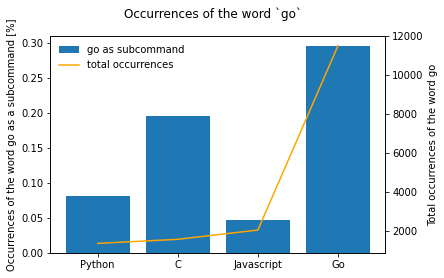
\includegraphics[width=8cm]{go_occ.png}
    \caption{Examined bigrams starting with \emph{go} and ending with a golang CLI subcommand. Also total occurrences are shown with the orange line.}
    \label{fig:go-occ}
\end{figure}

One can see (Fig. \ref{fig:go-occ}) that Go demonstrates a noticeable difference, which explains the often usage of the word \emph{go} by golang developers. Additionally, golang has a language keyword \texttt{go} which runs a function concurrently. This function is at the core of Golang, and is very likely to be discussed often by its developers.

It is interesting to see that even though the usage of the word \emph{go} by C developers is much rarer than by Golang developers, a big chunk of the occurrences (20\%) are in the context of a Golang CLI subcommand. To verify that the concordance of the word \emph{go} in the C class was checked. Mentions of \texttt{gccgo} and \texttt{cgo} can be noticed. These are respectively the GNU Golang compiler and the C interface for Golang programs. It would seem, that C developers are also Golang developers thus the increase use of the word go in the context of the CLI tool.

\subsection{Frequency of passive sentences}

Here POS tagging was used to classify sentences as passive or not. As expected, the frequency of passive sentences is high for all languages (in comparison to 10\% in most books), as it describes specific bugs in the code. One can see that C programmers use passive sentences the most, achieving almost 40\% of total passive sentences.

\begin{figure}[H]
    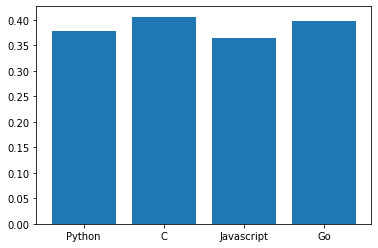
\includegraphics[width=8cm]{passives.png}
    \centering
\end{figure}

\subsection{Flesch readability score}

In our case, C and Go developers show a lower score than Python and Javascript. However all classes would be still classified in the 60-70 range, described as {\it Plain English. Easily understood by 13- to 15-year-old students} \cite{flesch}. This score takes into account number of syllables per word and sentence length, which, as established earlier, was not high in most cases.


\begin{figure}[H]
    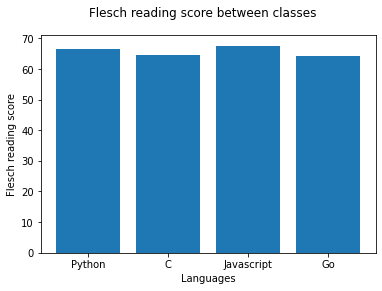
\includegraphics[width=8cm]{flesch.png}
    \centering
\end{figure}

\subsection{Flesch-Kincaid grade level}

In this case, all languages scored below 9. Similarly to the reading score, both C and Go issues rank higher therefore are deemed to be harder to understand.

\begin{figure}[H]
    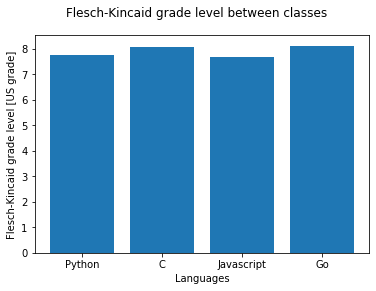
\includegraphics[width=8cm]{flesh_kincaid.png}
    \centering
\end{figure}

\subsection{Sentiment analysis}

Using NLTK's pretrained sentiment analyzer called VADER, each issue is assigned the compound sentiment intensity (in range $[-1; 1]$ where -1 represents the negative polarity, and +1 the positive one).

\begin{figure}[H]
    \centering
    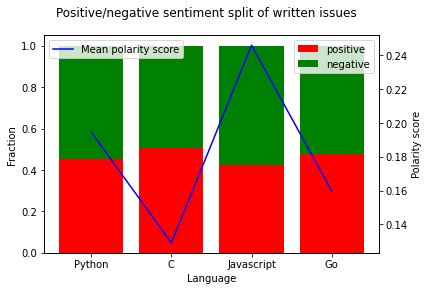
\includegraphics[width=8cm]{sentiment.png}
\end{figure}

C and Go issues exhibit a more negative sentiment. Since these languages are much more lower level compared to the other two, then we can expected them to be more frustrating which in turn causes the anger to be transferred onto GitHub issues. Additionally, C issues show the smallest total mean for the sentiment intensity, making it on average the most negative class of the four.

\subsection{Wordcloud}

For eye-candy purposes a wordcloud is constructed for each class with redacted common stopwords.

\begin{figure}[H]
    \centering
    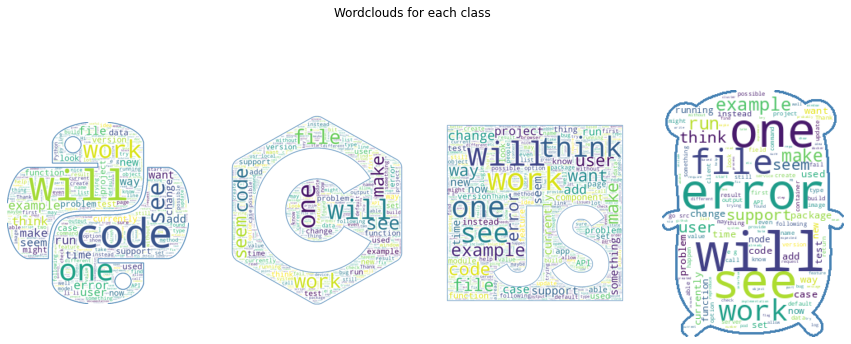
\includegraphics[width=\textwidth]{wordcloud.png}
    \caption{Wordclouds of all issues concatenated per class masked by the class language logo}
\end{figure}

No meaningful conclusions can be drawn from this. The only thing that caught our eye is the large \emph{error} word in the golang wordcloud. Possibly attributed to error being a first-party type in Golang\footnote{\url{https://pkg.go.dev/errors}}.

\newpage

\section{Conclusions}

As presented, gathered results were unfortunately underwhelming. In many cases classes showed very little variance. We believe that our aggressive normalization could negatively affect the final results. For example, we chose most popular Github users which possibly do not represent the real demographic for each class and only show the most advanced programmers. Often more advanced programmers are fluent in multiple programming languages which violates our isolation of classes. This was observed during word frequency distribution analysis where C programmers were also Golang programmers. In retrospection, we could have chosen a more representative group by for example choosing random users regardless of their popularity. We, however, feared to do so due to expected lower quality of posted issues. A different data source could be used too, perhaps dedicated programming language forums which should contain much more isolated data.

On the other hand, we do believe the shown results do point at some small, but existing difference. C and Go classes often scored as "more complex" in many different measured statistics. One could exploit these differences and build a feature map from them to then train a classifier.

Given the presented information, we conclude that differences in natural language complexity used by developers of different programming languages are too small to be statistically significant, but we do encourage a similar study to be performed on a much more controlled set of data.

\section{Attachments} \label{attachments}

\begin{enumerate}
    \item %SCRAPER_ZIP%
    \item %DATA_CLEANER_ZIP%
    \item %ANALYSIS_ZIP%
\end{enumerate}


\begin{thebibliography}{9}
    \bibitem{letterfreq}
    Peter Norvig (2012): \emph{English Letter Frequency Counts: Mayzner Revisited} \url{http://norvig.com/mayzner.html}

    \bibitem{flesch}
    Rudolf Flesch (1979): \emph{How to Write Plain English: A Book for Lawyers and Consumers}
\end{thebibliography}

\end{document}
